\documentclass[10pt,a4paper]{article}
\usepackage[margin=2.3cm]{geometry}
\usepackage{amsmath,amssymb}
\usepackage{booktabs,array,longtable,tabularx}
\usepackage{graphicx,float,caption}
\usepackage{xcolor}
\usepackage{listings}
\usepackage{enumitem}
\usepackage{tikz}
\usetikzlibrary{arrows.meta,positioning,calc}
\usepackage[colorlinks=true,linkcolor=teal!50!black,urlcolor=blue!50!black,citecolor=teal!50!black]{hyperref}
\usepackage{microtype}
\usepackage{seqsplit}
\emergencystretch=2em

\setlist{itemsep=2pt,topsep=3pt,parsep=0pt}
\captionsetup{font=small,labelfont=bf}
\setlength{\parindent}{0pt}
\setlength{\parskip}{5pt}
\renewcommand{\arraystretch}{1.12}

\definecolor{cgood}{HTML}{0F766E}
\definecolor{cbad}{HTML}{C2410C}
\lstset{basicstyle=\ttfamily\footnotesize,breaklines=true,frame=single,rulecolor=\color{black!25},
        backgroundcolor=\color{black!3},columns=fullflexible,keepspaces=true,showstringspaces=false}

\newcommand{\tx}[1]{\texttt{\detokenize{#1}}}
\newcommand{\txl}[1]{\texttt{\expandafter\seqsplit\expandafter{\detokenize{#1}}}}
\newcommand{\KLD}{\mathrm{KLD}}
\newcommand{\W}{\mathbf{W}}
\newcommand{\X}{\mathbf{x}}
\newcommand{\HD}{\mathbf{R}}

\title{\textbf{Q4-quality INT4 inference for Ossicle-4B on RDNA3: 10k prefill, 200\,tokens/s decode}\\[2pt]
\large Rotated GPTQ weights, 8-bit and 4-bit activations on WMMA, and what it cost\\[-2pt]
\normalsize A technical report on the full run: methods, measurements, failures}
\author{Work log compiled from the session logs, scripts and commits}
\date{2 November 2026}

\begin{document}
\maketitle
\thispagestyle{empty}

\begin{abstract}
\noindent
We take the Ossicle-4B audio--language model (Qwen3.5-4B backbone, Qwen3-Omni AuT audio encoder), convert it to GGUF for
llama.cpp, quantise it in ten standard formats, and then build a custom prefill/decode path for a single AMD RX~7900~XT
(RDNA3, \tx{gfx1100}) that stores every linear weight \emph{Hadamard-rotated}, \emph{GPTQ-quantised} to symmetric int4, and
multiplies it on the int4 WMMA units against rotated 8-bit or 4-bit activations.
A one-variable preset, \tx{GGML_INT4_PREFILL=fast}, reaches \textbf{10{,}690 tokens/s prefill at pp512 (10{,}648 at pp2048) with decode at
201.5\,tokens/s}, at KLD~0.101 against BF16 (Q3\_K\_L class by KLD, MMAU unchanged within noise): 2.3$\times$ the prefill of Q4\_K\_M (4{,}733) and 53\% faster decode.
The default \tx{quality} preset (one 2.55\,GB file, one copy of the weights in VRAM: 3.37\,GB peak) reaches 7{,}000 tokens/s at pp512 (7{,}020 at pp2048) with the same
201.5\,tokens/s decode at \textbf{KLD~0.025}, i.e.\ better agreement with BF16 than Q4\_K\_M (KLD~0.030--0.032) at about 50\% faster prefill.
Decode went from 92 to 201.5\,tokens/s almost entirely by removing kernel launches (847 $\to$ 236 per token, Sections~\ref{sec:final} and~\ref{sec:decode2}), followed
by two last latency changes in the matvec prologue and the attention combine. Multi-token-prediction speculative decoding on top of the
earlier 199\,tokens/s build reaches \textbf{229\,tokens/s} (output identical to plain decoding), and the same recipe applied to the stock Qwen3.5-4B gives
the same quality and speed.
We document every experiment, including the ones that failed (FP4 re-gridding, sparsity skipping, wider weight scale groups, the
256-wide WMMA attention kernel shipped upstream, and a dozen decode ideas in Section~\ref{sec:decode2}) and the caveats that remain.
\end{abstract}

\vspace{4pt}
\begin{center}
\small
\begin{tabular}{@{}lrrrrrr@{}}
\toprule
\textbf{Headline (RX 7900 XT, ROCm 10.1.0)} & pp512 & pp2048 & tg128 & KLD & same top-1 & MMAU\\
\midrule
Q4\_K\_M (best stock Q4, reference) & 4{,}733 & 4{,}595 & 131.6 & 0.032 & 91\% & 72.2\\
rotated INT4, \tx{fast} & \textbf{10{,}690} & \textbf{10{,}648} & \textbf{201.5}$^{\dagger}$ & 0.101 & 85.0\% & 71.8\\
rotated INT4, \tx{balanced}$^{\ddagger}$ & 9{,}398 & 9{,}109 & \textbf{201.5}$^{\dagger}$ & 0.070 & 88.1\% & --\\
rotated INT4, \tx{quality} (default) & 7{,}000 & 7{,}020 & \textbf{201.5}$^{\dagger}$ & 0.025 & 92.3\% & 71.7\\
\midrule
\tx{quality} + MTP (2 drafts, \tx{llama-server})$^{\S}$ & \multicolumn{2}{c}{--} & \textbf{229} & 0.025 & -- & --\\
\bottomrule
\end{tabular}\\[3pt]
\parbox{.92\linewidth}{\scriptsize $^{\dagger}$\tx{llama-bench} tg128 after a 128-token context (\tx{-d 128}); from an empty context the same build gives 199.7--200.1 (Q4\_K\_M: 131.6
from an empty context). Decode does not depend on the prefill preset. $^{\ddagger}$Prefill not re-measured since the earlier build. $^{\S}$Measured on the 199\,tokens/s build;
not re-run with the two newest decode patches.}
\end{center}

\tableofcontents
\newpage

%=====================================================================================================================
\section{Goal, hardware and model}
\label{sec:goal}

The work proceeded in a sequence of requests, each building on the last:
\begin{enumerate}
\item Convert the BF16 Ossicle-4B checkpoint to GGUF; quantise it in the usual llama.cpp formats; measure quality (perplexity,
      KL divergence, MMAU) and speed on an RX~7900~XT and an RTX~5060~Ti; push the result to a private HF repository.
\item Fix the audio front end of llama.cpp so GGUF accuracy matches PyTorch (opt-in GGUF keys), and move AMD to ROCm~10.1.
\item Use the 7900~XT's int4 matrix instructions for a faster prefill (a ``W4A4'' path).
\item \emph{``Get decode up and reduce KL vs BF16. Get it to Q4 quality.''}
\item \emph{``Get me 8k prefill with this decode.''}
\end{enumerate}
Items 4 and 5 are the focus of this report; items 1--3 are summarised (Sections~\ref{sec:baseline}--\ref{sec:wmma}) because
the later work depends on them.

\paragraph{Hardware and software.}
GPU: AMD Radeon RX~7900~XT (gfx1100, wave32, 20\,GB, 254\,W power cap, sustained clock $\approx$2.28\,GHz).
Second GPU for cross-checking the standard quants: NVIDIA RTX~5060~Ti 16\,GB (CUDA~13.0).
ROCm~10.1.0 from the pip wheels (isolated venv; ROCm~7.2.0 kept for comparison). llama.cpp fork
\tx{SILVERTHRONE32/llama.cpp-ossicle}, branch \tx{ossicle}, based on upstream \tx{f2b52a87e}; current head \tx{ad3d82c29} plus the two uncommitted decode patches of Section~\ref{sec:decode2}.

\paragraph{Model.}
The language model is Qwen3.5-4B (merged LoRA), 4.21\,B parameters: 32 layers, hidden size 2560, FFN width 9216, vocabulary
248{,}320 with tied embedding/head (1.27\,GB in BF16). Layers alternate three \emph{gated-delta-net} (GDN, linear-attention)
layers with one full-attention layer (24 GDN + 8 attention). GDN uses 16 key heads, 32 value heads, head dimension 128 and a
4-wide causal convolution; full attention uses 16 query heads, 4 KV heads, head dimension 256.
The 200 quantised linear tensors are, per layer kind: GDN \tx{attn_qkv}, \tx{attn_gate} (the z-gate), \tx{ssm_out}; attention
\tx{attn_q}, \tx{attn_k}, \tx{attn_v}, \tx{attn_output}; and in every layer \tx{ffn_gate}, \tx{ffn_up}, \tx{ffn_down}
($24\!\times\!3+8\!\times\!4+32\!\times\!3=200$).

\paragraph{Metrics.}
\begin{itemize}
\item \textbf{KLD / same-top-1}: \tx{llama-perplexity --kl-divergence} against logits of the BF16 GGUF on WikiText-2 test, context 512,
      24 chunks ($\approx$12k tokens). Standard error is about $\pm0.001$ near KLD~0.025 and $\pm0.003$ near 0.1.
\item \textbf{PPL}: WikiText-2 test, full set (standard quants) or the same 24 chunks (INT4 variants; stated as ``vs BF16'').
\item \textbf{MMAU}: test-mini, 1000 questions, greedy decoding through \tx{llama-server}, string-match scorer; standard error
      $\pm$1.4\,pp, so differences under $\sim$3\,pp are noise. PyTorch BF16 scores 72.1.
\item \textbf{Speed}: \tx{llama-bench}. For the INT4 work we use the \emph{median of 8 runs after discarding the first}
      (\txl{scripts/bench_med.sh}: \tx{-r 9}, first sample dropped), because the first sample is taken at cold GPU clocks and
      wrecks short means (e.g.\ one 3-run bench logged pp512 $4810\pm1416$ against a steady 5{,}846).
\end{itemize}

%=====================================================================================================================
\section{Baseline: GGUF conversion and the standard quant ladder}
\label{sec:baseline}

The BF16 safetensors were converted with llama.cpp's \tx{qwen35} text architecture and \tx{qwen3a} mmproj
(\txl{scripts/convert_ossicle.py}); the chat template is patched to always emit an empty \tx{<think>} block, which is how
Ossicle was trained. Ten quants were produced with an importance matrix from WikiText-2 train (Q8\_0 without) and each was
measured on both GPUs. Table~\ref{tab:quants} is the quality table, Table~\ref{tab:quantspeed} the speed table.

\begin{table}[H]
\centering\small
\caption{Standard quants of Ossicle-4B. PPL: WikiText-2 test. MMAU: patched llama.cpp (audio fix of Section~\ref{sec:audio}).}
\label{tab:quants}
\begin{tabular}{@{}lrrrrrrr@{}}
\toprule
Quant & GB & PPL & KLD & top-1 \% & MMAU XT & MMAU Ti & MMAU stock\\
\midrule
BF16 (ref) & 8.42 & 10.571 & -- & -- & 71.8 & 71.8 & 70.2\\
Q8\_0 & 4.48 & 10.566 & 0.0023 & 97.9 & 72.3 & 72.1 & 70.5\\
Q6\_K & 3.46 & 10.670 & 0.0063 & 95.6 & 72.3 & 72.4 & 70.5\\
Q5\_K\_M & 3.08 & 10.740 & 0.0146 & 94.0 & 72.8 & 72.2 & 71.2\\
Q4\_K\_M & 2.71 & 10.951 & 0.0303 & 91.1 & 72.1 & 72.4 & 70.0\\
Q4\_K\_S & 2.56 & 10.939 & 0.0346 & 90.8 & 72.0 & 71.9 & 70.8\\
Q4\_0 & 2.55 & 10.994 & 0.0581 & 89.2 & 71.9 & 71.7 & 70.8\\
IQ4\_XS & 2.51 & 10.884 & 0.0346 & 90.9 & 72.0 & 71.4 & 70.9\\
Q3\_K\_L & 2.42 & 11.681 & 0.1011 & 85.5 & 70.3 & 70.2 & 69.4\\
Q3\_K\_M & 2.26 & 11.820 & 0.1077 & 85.0 & 70.6 & 70.7 & 70.5\\
Q3\_K\_S & 2.07 & 12.203 & 0.1492 & 82.5 & 69.6 & 69.9 & 69.3\\
\bottomrule
\end{tabular}
\end{table}

\begin{table}[H]
\centering\small
\caption{Speed of the standard quants (first-token = full \tx{llama-server} path with one 10\,s clip; XT = 7900~XT/ROCm 10.1,
Ti = 5060~Ti/CUDA 13.0). These use a different method from the INT4 tables (server median of 5), hence Q4\_K\_M pp512 of 4{,}482
here against 4{,}733 in the INT4 comparisons.}
\label{tab:quantspeed}
\begin{tabular}{@{}lrrrrrr@{}}
\toprule
Quant & XT pp512 & XT first tok (ms) & XT tg (t/s) & Ti pp512 & Ti first tok (ms) & Ti tg (t/s)\\
\midrule
BF16 & -- & -- & -- & 3933 & 167 & 47.0\\
Q8\_0 & 4775 & 150 & 95.4 & 4971 & 139 & 81.2\\
Q6\_K & 4035 & 170 & 115.7 & 4141 & 136 & 98.6\\
Q5\_K\_M & 4484 & 150 & 120.2 & 4572 & 130 & 108.1\\
Q4\_K\_M & 4482 & 153 & 126.6 & 4653 & 128 & 119.0\\
Q4\_K\_S & 4552 & 144 & 129.5 & 4802 & 128 & 124.3\\
Q4\_0 & 4602 & 149 & 130.7 & 5033 & 121 & 128.5\\
IQ4\_XS & 4675 & 144 & 136.5 & 5035 & 122 & 127.9\\
Q3\_K\_L & 4109 & 152 & 127.7 & 4448 & 131 & 118.2\\
Q3\_K\_M & 4118 & 150 & 131.1 & 4441 & 129 & 123.3\\
Q3\_K\_S & 3905 & 154 & 132.8 & 4206 & 131 & 123.8\\
\bottomrule
\end{tabular}
\end{table}

Observations that shaped later decisions:
\begin{itemize}
\item KLD orders the quants cleanly; MMAU between Q8\_0 and IQ4\_XS (71.4--72.8) is inside noise, and only the Q3 family drops
      below the PyTorch reference. We therefore use KLD for ranking and MMAU as a sanity check.
\item Q4\_K\_M's prefill (about 4.5--4.7k t/s) is the number to beat; the llama.cpp INT8 MMQ path tops out near
      36--40 TOPS on this card.
\item Mixed-precision storage is cheap: the 1.27\,GB BF16 token-embedding/head tensor alone costs about 1\,ms per decoded
      token (Section~\ref{sec:decode}).
\end{itemize}

%=====================================================================================================================
\section{Audio front-end fix and ROCm 10.1}
\label{sec:audio}

\paragraph{Audio.} On stock llama.cpp the BF16 GGUF scores 70.2 on MMAU against 72.1 for PyTorch. Three differences in
the mtmd audio path were found and fixed as \emph{opt-in} GGUF keys (default off, so other models behave as upstream):
\txl{clip.audio.no_boundary_tokens} (Ossicle never saw \tx{<|audio_start|>}/\tx{<|audio_end|>}; $\approx$+1.2\,pp),
\txl{clip.audio.polyphase_resample} (Kaiser polyphase like \txl{scipy.signal.resample_poly} instead of linear; $\approx$+0.7\,pp)
and \txl{clip.audio.exact_frame_count} (\texttt{ceil(n/hop)} mel frames as \txl{WhisperFeatureExtractor}; $\approx$+0.3\,pp).
Patched BF16 reaches 71.8 (976/1000 answers identical to PyTorch). As a transfer check, the same two applicable keys lifted
Qwen3-Omni-30B-A3B (Q4\_K\_M) from 78.9 to 80.0 MMAU (+1.10$\pm$0.46\,pp paired, 16 up/5 down).

\paragraph{ROCm.} On ROCm~7.2.0, Q8\_0 and IQ4\_XS (pp512 $\approx$1{,}100--1{,}300) and short-batch Q4\_0 had slow
prefill; ROCm~10.1.0 fixes it (Q8\_0 pp512 1{,}123\,$\to$\,4{,}775) at the price of 1--3\% slower generation. All later work
uses 10.1.0.

%=====================================================================================================================
\section{Int4 WMMA microbenchmarks}
\label{sec:wmma}

RDNA3 exposes \texttt{v\_wmma\_i32\_16x16x16\_iu4} at \emph{twice} the rate of the iu8 variant. A pure-WMMA
microbenchmark sustains 182~TOPS (190 on paper; about 195 at the 2.28\,GHz this card holds at its power cap).

A standalone kernel was developed through 27 successive variants (\txl{kernel/q4k_iu4_v2} \ldots\ \txl{q4s_iu4_v27}), always
verified against a CPU reference (relative error $4.5\!\times\!10^{-4}$). The format: symmetric int4 weights (signed codes,
no zero point) with one integer sub-scale per 32/64/128 K-values, multiplied by int4 activations.

\begin{table}[H]
\centering\small
\caption{Standalone int4 GEMM throughput after warm-up (FFN $9216\times2560$ at $N=512$; down $2560\times9216$ at $N=2048$).}
\begin{tabular}{@{}lrrrr@{}}
\toprule
Sub-scale per & FFN $N{=}512$ & FFN $N{=}2048$ & down $N{=}2048$ & extra KLD vs per-32\\
\midrule
32 K-values & 125 TOPS & 128 & 124 & --\\
64 & 142 & 144 & 143 & +0.011\\
128 & \textbf{149} & \textbf{149} & \textbf{152} & +0.015\\
\bottomrule
\end{tabular}
\end{table}
That is 78\% of the sustained theoretical peak and 83\% of the best pure-WMMA loop. Where the rest goes: fragment loads
$\approx$8--10\%, integer scaling $\approx$5\%, loop structure $\approx$4\%. At llama.cpp's own reference shape
(Q4\_K, $M{=}4096$, $N{=}512$, $K{=}14336$) the pipeline ``fused Hadamard rotation + quantise (0.04\,ms) + GEMM (0.43\,ms)''
takes 0.47\,ms (128 TOPS end-to-end) against 1.52\,ms (39.6 TFLOPS in \tx{test-backend-ops}) for the existing INT8 MMQ,
i.e.\ about 3.2$\times$ on the matmul.

What got there: operand-ready weight repacking; scalar buffer-load addressing; 24-bit integer multiply-adds (inline asm);
8+ independent WMMA chains with scheduler barriers; chaining the accumulator through a whole scale unit (one multiply-add per
unit); arranging a block's waves along the token dimension (1$\times$8 waves so the weight tile is shared through cache);
and a fused one-pass rotate+quantise+pack kernel (HadaCore idea, own RDNA3 implementation).

\paragraph{Benchmark pitfall.} With only $\sim$10\,ms of launches the GPU never reaches full clocks and a kernel looks about
1.5$\times$ slower (71 vs 110 TOPS for the same kernel). Warm up for at least 1\,s of load. The same effect is why the
\tx{llama-bench} medians drop the first sample.

\paragraph{Dead ends in the microbenchmark phase.}
\begin{itemize}
\item \textbf{FP4 checkpoints.} E2M1 needs 5 bits once doubled, so it cannot go through one int4 pass exactly. Re-fitting
      NVFP4/MXFP4 weights onto a uniform int4 grid cost about +0.07 KLD (0.096 native $\to$ 0.16--0.19). Plain symmetric int4
      from a BF16 source is as accurate as FP4 (0.082 vs 0.098).
\item \textbf{Sparsity skipping.} A wave-uniform group-skip loop is exact (62\,$\to$\,98 TOPS at 75\% skipped) but real
      activations give almost nothing to skip: all-zero 16-token$\times$32-value tiles are 0--0.3\% lossless and 2--6\% even
      under aggressive thresholds (\txl{int4/sparsity_probe*.py}).
\end{itemize}

%=====================================================================================================================
\section{The rotated-INT4 format}
\label{sec:format}

\subsection{Rotation}
Four-bit \emph{activations} are the quality risk: transformer activations have outlier channels. We rotate with a
block-Hadamard transform. For a linear layer $y=\W\X$ with input dimension $K$ (multiple of 256), define per 256-block
\[
  \HD = \tfrac{1}{16}\,H_{256}\,D,\qquad D=\mathrm{diag}(s_j),\quad s_j=-1\ \text{if}\ \big((j\cdot 2654435761)\bmod 2^{32}\big)\gg 31,\ \text{else}\ +1,
\]
where $H_{256}$ is the Sylvester Hadamard matrix. $\HD$ is orthogonal, so $\W'=\W\HD^{\!\top}$ (applied blockwise along $K$) and
$\X'=\HD\X$ give $\W'\X'=\W\X$ exactly. The weights are rotated \emph{offline} (\tx{scripts/rotate_quantize.py}); activations
are rotated \emph{online} in the backend. The sign pattern is a hash so the C++ side and the converter agree without storing it.
Rotation Gaussianises both operands, which is what makes 4-bit codes viable.

\subsection{GPTQ on the rotated weights}
The initial files used round-to-nearest (RTN) with $|\max|/7$ scales and codes in $[-7,7]$. The final files use GPTQ
(\tx{scripts/gptq_rotate.py}):
\begin{enumerate}
\item Load the Ossicle LM in transformers (from \tx{stage_lm} and the \tx{src/} safetensors), BF16 on GPU.
\item Register a forward pre-hook on each of the 200 target linears; for the rotated input $\X'$ (in llama.cpp column order,
      including the out-projection head re-order) accumulate $H=\sum \X'^{\!\top}\X'$ in fp32 on the CPU.
      Calibration: 128 sequences $\times$ 512 tokens of WikiText-2 \emph{train}, batches of 8.
\item For each tensor, GPTQ with Cholesky-inverse error feedback (damping 0.01 of the mean diagonal, column blocks of 128),
      codes in $[-8,7]$, one fp16 scale per group of 32 columns. Each group's scale is chosen on the error-compensated
      weights by an MSE search over 26 candidates $\{0.55,\ldots,1.05\}\cdot\max|w|/7$, rounded to fp16.
\item Pack as ordinary \textbf{Q4\_0 blocks} (fp16 scale + 16 bytes: element $j$ low nibble, $j{+}16$ high nibble) in a
      safetensors file keyed by GGUF tensor name. No new GGUF type is introduced.
\item \tx{rotate_quantize.py --blocks} rebuilds the GGUF from BF16, re-rotating each tensor and \emph{asserting the dequantised
      blocks are within 0.25 relative error of it} (a wrong row/column order shows up as $\approx$1.0).
\end{enumerate}
GPTQ runs end-to-end in about four minutes (Hessians + 200 tensors; the quantisation loop itself $\approx$106\,s) and
about 15\,GB of RAM. Mean relative weight error: 0.1071 (group 32), 0.1179 (group 64). A group-128 run was not completed and was dropped.

The token embedding/output head is requantised separately: Q6\_K (via \tx{ggml_quantize_chunk}) or Q8\_0. The GGUF gains two keys,
\txl{ossicle.int4_rotation_block}=256 and \txl{ossicle.int4_scale_group}; the loader sets \tx{GGML_INT4=3} automatically when
the first is present.

\subsection{How much does each ingredient buy?}
Because iterating on the real runtime is slow, a Hugging Face simulation (\txl{int4/w4a4_sim2.py}; Qwen3.5-4B, 24 chunks of
512 tokens, fake-quantised linears with exactly the rotation, scale-group and activation-scale logic of the kernels) was used to
find what recovers quality. Figure~\ref{fig:ladder} gives the ladder; the simulation's absolute KLD differs from the real file
by a few thousandths because it quantises in bf16 matmuls and uses a different text slice.

\begin{figure}[H]
\centering\includegraphics[width=.82\linewidth]{fig/ladder.pdf}
\caption{Simulated KLD ladder. The quality killer is the 4-bit \emph{activation}, not the 4-bit weight: with GPTQ weights,
8-bit activations (0.029) are indistinguishable from 16-bit (0.029), while 4-bit activations cost +0.095.}
\label{fig:ladder}
\end{figure}

Complete simulation results (KLD against fp16, same-top-1 in parentheses; fp16 PPL 11.560):
\begin{center}\small
\begin{tabular}{@{}lr@{}}
\toprule
Configuration & KLD (top-1 \%)\\
\midrule
RTN, scale/128, A4 & 0.2195 (77.6)\\
RTN, scale/128, A16 & 0.1125 (84.5)\\
MSE, scale/128, A16 & 0.0807 (86.4)\\
MSE, scale/64, A16 & 0.0686 (87.1)\\
MSE, scale/32, A16 & 0.0584 (88.3)\\
MSE, scale/32, A4 & 0.1549 (81.5)\\
MSE, scale/32, A8 & 0.0588 (88.1)\\
MSE, scale/32, A16, 8-bit \tx{down} weights & 0.0477 (89.1)\\
MSE, scale/32, A16, 8-bit \tx{down+v+o+ssm} weights & 0.0294 (91.3)\\
GPTQ, scale/32, A16 & 0.0289 (92.2)\\
GPTQ, scale/32, A8 & 0.0294 (92.2)\\
GPTQ, scale/32, A4 & 0.1243 (83.3)\\
GPTQ, scale/32, A4 except A8 on \tx{down+o+ssm} & 0.0845 (86.1)\\
\bottomrule
\end{tabular}
\end{center}
Three conclusions: (i)~scale-per-32 beats per-64/128 by 0.01--0.02 KLD; (ii)~GPTQ is worth about 0.03 KLD over MSE scales;
(iii)~A8 is free, A4 is not.

%=====================================================================================================================
\section{Runtime: the activation paths}
\label{sec:runtime}

\begin{figure}[H]
\centering
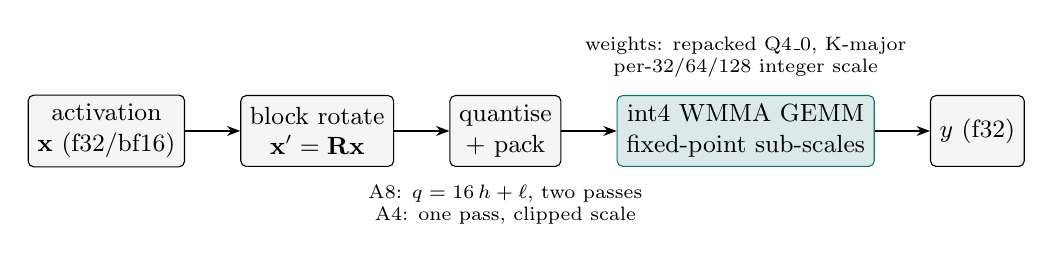
\begin{tikzpicture}[node distance=7mm,>=Stealth,
  box/.style={draw,rounded corners=2pt,minimum height=9mm,align=center,font=\small,fill=black!4},
  hot/.style={box,fill=cgood!15,draw=cgood}]
\node[box] (x) {activation\\$\X$ (f32/bf16)};
\node[box,right=of x] (r) {block rotate\\$\X'=\HD\X$};
\node[box,right=of r] (q) {quantise\\+ pack};
\node[hot,right=of q] (g) {int4 WMMA GEMM\\fixed-point sub-scales};
\node[box,right=of g] (y) {$y$ (f32)};
\draw[->] (x)--(r); \draw[->] (r)--(q); \draw[->] (q)--(g); \draw[->] (g)--(y);
\node[font=\scriptsize,below=1mm of q,align=center] {A8: $q=16\,h+\ell$, two passes\\A4: one pass, clipped scale};
\node[font=\scriptsize,above=1mm of g,align=center] {weights: repacked Q4\_0, K-major\\per-32/64/128 integer scale};
\end{tikzpicture}
\caption{Prefill GEMM pipeline for a rotated tensor (rotate, quantise and pack are one fused kernel).}
\end{figure}

\subsection{Eight-bit activations on int4 hardware (default prefill, ``quality'')}
Every int8 code $q\in[-128,127]$ is split as $q=16h+\ell$ with $h\in[-8,7]$ signed and $\ell\in[0,15]$ unsigned. The GEMM
runs the $h$ pass, shifts the integer accumulator by 4 bits, runs the $\ell$ pass into the \emph{same} accumulator, and then
applies the integer weight sub-scale. Two int4 passes cost the same as one int8 pass, but the iu4 pipe is the one that is twice
as fast, so the effective rate is 134 int4-TOPS $=$ 67 int8-equivalent TOPS (about 74\% of the iu4 ceiling) against 36--40 TOPS
for the stock INT8 MMQ path. Integer weight scales use a fixed-point shift (SH8 $=12$), and the final cross-unit accumulation is
carried in float to avoid 24-bit overflow in the integer multiply-adds.

The weight scale group is detected at load time (\tx{k_detect_gw}: GW $\in\{1,2,4\}$ means 32/64/128 columns per scale), so
the same kernel serves group-32, 64 and 128 files; group~64 gives about +5\% prefill for KLD 0.029 (0.0228 at group 32 with
the Q8 head), group 128 would be about KLD 0.04.

\subsection{Four-bit activations (the ``fast'' path)}
A single int4 pass, with the activation scale per 256-block expressed as a multiplier $m\in\{1,\ldots,16\}$ of $1/16$ of a
per-token reference scale: $m_b=\lceil 16\,\mathrm{clip}\cdot\mathrm{amax}_b/\mathrm{amax}_{\text{token}}\rceil$ (this mirrors the
simulation's \tx{act_quant}). Weight scales use SH $=10$. The \textbf{clip} factor shrinks the quantiser range so rare outliers
saturate instead of stretching the scale:

\begin{figure}[H]
\centering\includegraphics[width=.55\linewidth]{fig/clip.pdf}
\caption{Effect of the 4-bit activation clip (all tensors A4; KLD vs BF16). The default 0.85 reduced KLD from 0.113 to 0.092
at no cost in speed; 0.6 is too aggressive.}
\label{fig:clip}
\end{figure}

\subsection{Choosing activation width per tensor kind}
Environment variables select which tensors take the 4-bit path; everything else stays at 8 bit.
\begin{table}[H]
\centering\small
\caption{Control surface of the INT4 backend.}
\begin{tabularx}{\linewidth}{@{}lX@{}}
\toprule
Variable & Meaning\\
\midrule
\tx{GGML_INT4=1/2/3} & 1: rotation only; 2: 4-bit activations everywhere; 3: 8-bit activations (auto-set by the loader for rotated files)\\
\tx{GGML_INT4_PREFILL} & \tx{quality} (default): no A4; \tx{balanced}: A4 on \txl{attn_q.weight,attn_k,attn_v,attn_qkv,attn_gate,ffn_gate,ffn_up}; \tx{fast}: A4 on \tx{attn_,ffn_,ssm_}\\
\tx{GGML_INT4_A4=<substrings>} & explicit list of tensor-name substrings that use A4 (overrides the preset)\\
\tx{GGML_INT4_CLIP} & 4-bit activation clip factor, default 0.85\\
\bottomrule
\end{tabularx}
\end{table}

Per-kind sensitivity (simulation with GPTQ weights; baseline KLD 0.0269; Figure~\ref{fig:kinds}) shows why one cannot rescue
speed with a clever per-layer mix: the FFN has the FLOPs \emph{and} the sensitivity.

\begin{figure}[H]
\centering\includegraphics[width=.8\linewidth]{fig/kinds.pdf}
\caption{Added KLD when one tensor kind alone moves to 4-bit activations. FFN down/up/gate and the GDN out-projection dominate.}
\label{fig:kinds}
\end{figure}

%=====================================================================================================================
\section{Decode: from 92 to 132 tokens/s}
\label{sec:decode}

The first working INT4 path decoded at only 91.9\,t/s with the older RTN file. Diagnosis and fixes:
\begin{itemize}
\item \textbf{Decode is launch-bound, not bandwidth-bound.} The GPU is about 64\% busy with $\sim$3\,\textmu s gaps between
      $\sim$620 kernels per token; the matvec kernels already stream at the $\sim$733\,GB/s ceiling. So the lever is fewer and
      leaner kernels, not faster matvecs.
\item \textbf{Keep CUDA graphs and matmul fusion enabled.} The INT4 hook had disabled them; they are now skipped only for a rotated
      weight that cannot take the fused path (\txl{ggml_cuda_int4_fused_ok}).
\item \textbf{Fuse the rotation into Q8\_1 quantisation} for batches $\le 8$ (\tx{k_rot_q8_1}, called from \txl{mul_mat_vec_q}):
      one kernel instead of rotate-then-quantise. Decode always uses 8-bit activations, so it carries no A4 penalty.
\item \textbf{Shrink the head.} The 1.27\,GB BF16 tied embedding/head cost about 1\,ms per token alone. Q6\_K costs +0.002 KLD and
      buys +6 t/s; Q8\_0 is KLD-better (0.0228) but slower (126.6 t/s).
\end{itemize}
Result: 132.6 t/s (Q6\_K head) / 126.6 t/s (Q8\_0 head), against 131.6 t/s for Q4\_K\_M. All preset changes later in the work left
tg128 within 130--132.

%=====================================================================================================================
\section{Results: Q4-quality at higher prefill}
\label{sec:q4}

Median of 8 runs after the first; KLD on 24 chunks of WikiText-2 test; MMAU with the audio patch.

\begin{table}[H]
\centering\small
\caption{Rotated-INT4 files vs Q4\_K\_M (RX 7900 XT, ROCm 10.1.0, 8-bit prefill activations).}
\begin{tabular}{@{}lrrrrrrrr@{}}
\toprule
Model & GB & pp512 & pp2048 & tg128 & PPL vs BF16 & KLD & top-1 & MMAU\\
\midrule
Q4\_K\_M & 2.7 & 4{,}733 & 4{,}595 & 131.6 & +3.3\% & 0.032 & 91\% & 72.2\\
rotq4-gptq (Q6\_K head) & 2.55 & \textbf{5{,}571} & \textbf{5{,}399} & \textbf{132.6} & +1.9\% & 0.0246 & 92.2\% & 71.7\\
rotq4-gptq-q8head & 2.70 & 5{,}622 & 5{,}402 & 126.6 & +1.7\% & 0.0228 & 93.5\% & 72.0\\
\emph{older:} rotq4g4 (RTN, A4) & 3.3 & 8{,}041 & 7{,}615 & 91.9 & +17.6\% & 0.197 & 81\% & 69.0\\
\bottomrule
\end{tabular}
\end{table}
So the answer to ``get it to Q4 quality'' is positive: prefill $+18\%$ at that point, decode at par, and KLD \emph{below}
Q4\_K\_M's (0.023--0.025 vs 0.032), with MMAU inside noise of Q4\_K\_M and BF16.
The group-64 variant with the Q8 head gave KLD 0.0293 (so group-32 stays the default).
Note that 0.0246 above is from before the wave32 GDN kernel of Section~\ref{sec:gdn}; the same file measures 0.0252 after it
(floating-point summation order changes; the difference is inside the $\pm$0.0012 standard error).

%=====================================================================================================================
\section{Reaching 8k prefill}
\label{sec:8k}

The target: pp512 $\approx$ 8{,}000 tokens/s with decode held at $\sim$132 t/s. The 8-bit GEMM pair of passes is itself
close to its ceiling (Section~\ref{sec:tile}), so the remaining levers were (a)~use fewer GEMM bits per tensor, (b)~speed up
the non-GEMM parts (gated-delta-net recurrence first), (c)~recover the quality of (a).

\subsection{Per-kind A4 sweep}
\tx{scripts/sweep_a4.sh} runs, for each activation-width configuration of the \emph{same} GGUF, KLD (24 chunks) and
the median bench. Results (Figure~\ref{fig:pareto} plots them against the standard quants):

\begin{table}[H]
\centering\small
\caption{Prefill preset sweep on \protect\txl{ossicle-4b-gptq-g32-q6e.gguf}. Tokens/s are medians; ``A4 on'' lists the tensor kinds using
single-pass 4-bit activations (clip 0.85); the rest are A8.}
\label{tab:sweep}
\begin{tabular}{@{}lrrrrr@{}}
\toprule
A4 on & pp512 & pp2048 & tg128 & KLD & top-1 \%\\
\midrule
nothing (\tx{quality}) & 5{,}846 & 5{,}647 & 131.8 & 0.0252 & 92.5\\
q/k/v, qkv, z-gate, ffn gate & 6{,}784 & 6{,}488 & 131.9 & 0.0519 & 89.3\\
\;+ ffn up (\tx{balanced}) & 7{,}257 & 6{,}935 & 131.5 & 0.0713 & 87.3\\
\;+ ffn down & 7{,}857 & 7{,}504 & 131.3 & 0.0871 & 86.8\\
everything (\tx{fast}) & \textbf{8{,}248} & 7{,}797 & 131.9 & 0.0964 & 85.4\\
\bottomrule
\end{tabular}
\end{table}

\begin{figure}[H]
\centering\includegraphics[width=.9\linewidth]{fig/pareto.pdf}
\caption{Prefill speed against fidelity. Stock quants cluster at 4.0--4.8k t/s; the rotated-INT4 sweep moves right along a roughly
linear speed--KLD trade-off from 5.8k to 8.2k. (Stock KLD from the full-study table; INT4 points from the sweep above.)}
\label{fig:pareto}
\end{figure}

The final confirmation run of \tx{fast} on the committed build gave pp512 8{,}269 / pp2048 7{,}802 / tg128 131.7 (the sweep run
measured 8{,}248 / 7{,}797 / 131.9; run-to-run variation is $\sim$0.3\%). Likewise the \tx{balanced} confirmation gave
pp512 7{,}243 / pp2048 6{,}930 against the sweep's 7{,}257 / 6{,}935. We quote the final numbers in the abstract and the sweep
numbers in this table; neither is a transcription error.

\begin{table}[H]
\centering\small
\caption{Final presets, same file (\tx{rotq4-gptq}, Q6\_K head).}
\begin{tabular}{@{}lrrrrrrr@{}}
\toprule
Preset & pp512 & pp2048 & tg128 & PPL vs BF16 & KLD & top-1 & MMAU\\
\midrule
\tx{quality} (A8 everywhere) & 5{,}846 & 5{,}647 & 131.8 & +1.9\% & 0.0252 & 92.5\% & 71.7\\
\tx{balanced} & 7{,}243 & 6{,}930 & 131.1 & -- & 0.071 & 87.3\% & --\\
\tx{fast} (A4 everywhere) & \textbf{8{,}269} & \textbf{7{,}802} & \textbf{131.7} & +7.4\% & 0.096 & 85.4\% & 71.6\\
\bottomrule
\end{tabular}
\end{table}

\paragraph{Reading the trade-off.} \tx{fast} sits between Q4\_0 (KLD 0.058) and Q3\_K\_L (0.101) on KLD at about twice the
Q3 prefill rate. Its MMAU score (71.6) is indistinguishable from \tx{quality} (71.7), but MMAU has $\pm1.4$\,pp noise and
audio questions are dominated by the audio encoder; the KLD/PPL numbers are the more sensitive indicators and they do degrade.
Four-bit activations carry about 10\% relative noise per matmul (20\,dB SNR); at 8k the KLD cannot be recovered without
more bits.

\subsection{Where the speed comes from}
\begin{itemize}
\item \textbf{GEMM bit-width}: one pass instead of two for A4 tensors (the bulk of the 5{,}846\,$\to$\,8{,}269 gain).
\item \textbf{Activation clip 0.85}: quality only (KLD 0.113\,$\to$\,0.092 in the clip experiment), no speed effect.
\item \textbf{Wave32 gated-delta-net kernel}: $+5\%$ prefill (5{,}571\,$\to$\,5{,}846 at pp512), Section~\ref{sec:gdn}.
\end{itemize}

\subsection{Tile shapes}
\label{sec:tile}
The GEMM tile constants (MI$=$2, NJ$=$2, WAVES\_N$=$8) were varied: (2,2,4), (2,2,16) and (1,2,8) all landed within 2\% of
each other. The prefill GEMM is therefore near its practical ceiling (about 74\% of iu4 peak at A8), and the rest of the
prefill budget is no longer the GEMM alone: at \tx{fast}, a 512-token pass takes $\approx$62\,ms of which gated-delta-net is
22\%, flash attention 3--7\%, and rotate+quantise $\approx$3\%.

%=====================================================================================================================
\section{Gated-delta-net: what worked and what did not}
\label{sec:gdn}

The recurrence per head is $S_t = a_t\,S_{t-1} + k_t\,\delta_t^{\!\top}$ with $\delta_t = \beta_t\,(v_t - S_{t-1}^{\!\top}k_t)$ and
output $o_t=S_t^{\!\top}q_t$; state $S\in\mathbb{R}^{128\times128}$ per head, 24 GDN layers, 32 value heads. It is
sequential in $t$, and at pp512 it takes 0.54\,ms per layer per 512 tokens (22\% of a \tx{fast} pass).

\subsection{Kept: two lanes per state column (wave32)}
\tx{gated_delta_net_cols} (HIP only, $S_v{=}128$, scalar gate, non-KDA): each state column is owned by \emph{two} lanes holding
64 state registers each; one \texttt{\_\_shfl\_xor(\ldots,16)} per reduction; $k$/$q$ double-buffered in wave-private LDS; the next token's
$v,\beta,g$ prefetched. Grid $(H, n_{\text{seqs}}, 2)$, block $(32,4)$. Gain: +5\% prefill (pp512 5{,}571\,$\to$\,5{,}846), KLD unchanged
within error. The path that led here:
\begin{itemize}
\item Software pipelining of the original kernel's loads: no gain.
\item One lane per column: 256 VGPRs, spilled. LDS-staged variant: worse. \emph{Two} lanes per column (64 state registers each): fixed it.
\item Prefetching $v,\beta,g$ in the new kernel: no measurable gain.
\end{itemize}

\subsection{First attempt, reverted: chunked WY form without matrix instructions}
The chunked form turns the recurrence into matrix products per chunk of $C$ tokens: build the strictly lower-triangular
interaction $L$, invert $(I+L)$, form $\eta=U-W S_0$, produce the chunk's outputs, and update the state. A scalar-code prep and scan
kernel were \emph{correct} (KLD 0.0249 against 0.0252) but slower (3{,}401--5{,}307 against 5{,}846 tokens/s at pp512): without matrix
instructions the chunk algebra is bound by LDS latency and register pressure. That work was reverted and saved as
\txl{kernel/gated_delta_net_chunked_wip.cu}.

\subsection{Kept: chunked WY form on WMMA (Section~\ref{sec:final})}
The rewrite on \tx{v_wmma_f32_16x16x16_f16} is described in Section~\ref{sec:final}; the per-layer cost of the op fell from 0.46\,ms
to 0.14\,ms per 512 tokens (13\% $\to$ 4\% of a pass). The lesson of the first attempt carried over: on RDNA3 the code that decides
the speed is the \emph{ISA}, not the algebra --- twice the slowdown came from the compiler turning an unrolled \texttt{if (tok < n)
x = load(...)} into a branch with a \texttt{vmcnt(0)} wait per element, which serialises every global load.

%=====================================================================================================================
\section{Final round: one copy of the weights, WMMA gated-delta-net and attention, fusion, decode, MTP}
\label{sec:final}
This section supersedes the speed tables of Sections~\ref{sec:gdn}--\ref{sec:neg} written before it (the model, the
quantisation and the quality numbers are unchanged). All speeds: median of 8 \tx{llama-bench} runs after one discarded, RX 7900 XT. Decode was optimised further after this section was written: Section~\ref{sec:decode2} carries the final decode numbers.

\subsection{VRAM: 2$\times$ $\to$ 1$\times$}
The prefill kernel's repacked weight layout (nibbles in WMMA operand order plus fixed-point sub-scales) has \emph{exactly} the byte
size of the Q4\_0 tensor. Each rotated weight is therefore converted in place the first time a graph uses it, through a temporary copy
of one tensor at a time and before any CUDA graph is captured; decode got its own matvec (\tx{k_mv}) reading that layout directly, and
the GEMM accepts any contiguous batch shape. Peak VRAM for pp512+tg: 5{,}511\,$\to$\,3{,}413\,MiB (Q4\_K\_M: 3{,}652). Prefill
unchanged, decode +4\%, KLD bit-identical in prefill. This also exposed that the earlier \tx{fast} KLD was understated (Caveats).

\subsection{Prefill}
\begin{center}\small
\begin{tabular}{@{}p{7.4cm}rrrr@{}}
\toprule
 & \multicolumn{2}{c}{\tx{quality}} & \multicolumn{2}{c}{\tx{fast}}\\
step & pp512 & pp2048 & pp512 & pp2048\\
\midrule
start of this round (in-place weights) & 5{,}836 & 5{,}644 & 8{,}212 & 7{,}773\\
chunked WMMA gated-delta-net & 6{,}369 & 6{,}106 & 9{,}208 & 8{,}721\\
shared activation packing, SWIGLU / SILU$\cdot$mul inside the pack kernel, tiled conv concat & 6{,}744 & 6{,}489 & 10{,}090 & 9{,}501\\
WMMA flash attention (head 256), residual add in the GEMM epilogue, skinny bf16 gate kernel & 6{,}945 & 6{,}885 & 10{,}457 & 10{,}333\\
gate epilogue, paired q/k L2 norm, 128-thread head norms & 7{,}082 & 6{,}991 & 10{,}895 & 10{,}570\\
final (after the decode work) & \textbf{7{,}109} & \textbf{6{,}996} & \textbf{10{,}932} & \textbf{10{,}599}\\
\bottomrule
\end{tabular}
\end{center}
Perplexity, KLD (0.0250, +2.0\%) and MMAU (71.7--71.9) did not move beyond noise at any step; the fusions are bit-identical to the unfused
path, the GDN and attention kernels differ at the f16 level (below).

\paragraph{Chunked GDN on WMMA.} A \emph{prep} kernel (parallel over chunk$\times$head) forms $A=\mathrm{tril}(\beta_j e^{g_j-g_i}k_j\!\cdot\!k_i)$
and $P=\mathrm{tril}(e^{g_t-g_j}q_t\!\cdot\!k_j)$ with f16 WMMA, solves $(I+A)X=[\beta v\,|\,\beta e^{g}k]$ in 16-row panels (WMMA for the off-diagonal
updates, f32 for the 16$\times$16 diagonal solves) and stores $U$, $W$, $Q_g$, $K_d$, $P$; a \emph{scan} kernel (sequential over chunks,
parallel over heads $\times$ 16 state columns) keeps the f32 state in WMMA accumulators and does $\delta=U-WS$, $o=Q_gS+P\delta$,
$S\leftarrow e^{g_C}S+K_d^{\!\top}\delta$. 0.46\,ms $\to$ 0.14\,ms per layer per 512 tokens. Accuracy against an f64 recurrence on captured real
operands: $1.6$--$2.5\cdot10^{-4}$ relative RMS per layer (the per-token kernel: $4.5\cdot10^{-7}$). Because the 4/8-bit activation
quantisers amplify any perturbation, final logits differ from the per-token kernel's by KLD 0.002 (97\% same top-1), yet KLD against BF16 is
unchanged. A residual-bit variant (\tx{GGML_GDN_CHUNK=2}) did not help. Optimisation story: the first version took 167\,\textmu s per call; ISA inspection
showed \texttt{s\_waitcnt vmcnt(0)} after every load because loads sunk into predicated branches, an f32 triangular solve limited by LDS latency, and
SGPR spills. The panel scheme with branch-free preloads reached 93\,\textmu s; the scan 42\,\textmu s.

\paragraph{WMMA flash attention for head size 256.} The generic tile kernel ran at $\sim$14 TFLOPs and was 12.5\% of a \tx{fast} pp2048 pass.
Enabling upstream's own WMMA kernel for head 256 on RDNA3 gives wrong results (errors $\sim10^{-2}$; it is excluded upstream), so we wrote one
(\txl{fattn-rdna3.cu}): a block owns 64 rows = tokens$\times$GQA heads sharing a K/V head, 8 waves (the head dimension split over wave pairs, halving the
$O$ accumulators), Q in LDS, K and V$^{\!\top}$ tiles of 32 positions through one LDS buffer with conflict-free transposed V writes, K/V/mask
prefetched into registers, tiles fully hidden by the mask skipped, heaviest causal blocks scheduled first. 25.5\,ms $\to$ 12.0\,ms per pp2048 pass;
all 2{,}920 \tx{FLASH_ATTN_EXT} tests pass.

\paragraph{Fusion.} At pp2048 CUDA graphs cannot be reused (K/V length changes every ubatch), so every launch costs $\sim$3.3\,\textmu s of idle GPU. Folded
away: the three memsets per GEMM; the re-pack of activations shared by sibling matmuls (qkv+z, q/k/v, gate/up); SWIGLU / SILU$\cdot$mul feeding a GEMM (inside the pack kernel);
the residual ADD (GEMM epilogue); GDN alpha/beta (convert + hipBLASLt + convert $\to$ one skinny bf16 WMMA kernel with the sigmoid / softplus$\cdot A$ epilogue); the q/k L2 norms
(paired launch); the conv concat (tiled LDS transpose, 1.8\,ms $\to$ 0.6\,ms).

\subsection{Decode: 138 $\to$ 174 tokens/s}
A decode token needs $\approx$2.0\,GB of body weights plus the 0.52\,GB Q6\_K head: 3.4\,ms at the 750\,GB/s streaming ceiling. The profile showed 847
kernels per token with the GPU busy only 64\% of the time (a GDN layer: 26 kernels, 153\,\textmu s of work spread over 235\,\textmu s): the matvecs
already ran at $\sim$92\% of the ceiling, so the work was removing launches.
\begin{center}\small
\begin{tabular}{@{}p{10.5cm}rr@{}}
\toprule
step & kernels/token & tg128\\
\midrule
start & 847 & 138.3\\
rotated activations shared by sibling matvecs; residual add in the matvec epilogue & 732 & 143.3\\
GDN alpha/beta skinny bf16 matvec with gate epilogue (sigmoid; softplus$\cdot A$) & 708 & 147.1\\
RMS norm fused with the rotation + 8-bit quantisation (\tx{k_rmsnorm_rot_q8x}); silu(z)$\cdot$norm folded into the matvec rotation & 620 & 152.3\\
10-wave matvec blocks (divides the 10 superblocks of K=2560) & 620 & 155.0\\
GDN state read straight from the cache row (2\,MB gather per layer skipped) & 596 & 159.6\\
conv cluster: state gather + concat + cpy + \tx{ssm_conv} + silu in one kernel & 524 & 166.9\\
alpha+beta in one launch; q/k L2 norm folded into the GDN decode kernel & 476 & 172.3\\
rotation + quantisation inside the matvec for single-consumer inputs & 412 & 173.9\\
\bottomrule
\end{tabular}
\end{center}
Decode-path KLD/PPL are unchanged (batch 1: 0.0232, +1.87\%; batch 8: 0.0228, +1.78\%; MMAU 71.7). Two bugs worth recording: fusion bookkeeping keyed by tensor
addresses must be reset for every graph (the allocator reuses addresses; a stale entry turned into an assertion in the parallel server), and a fusion that executes a
later node early is only safe when nothing that allocates temporary memory sits in between (checked per pattern). What remains of a 5.7\,ms token:
matvecs 3.0\,ms, head 0.66\,ms (at the ceiling), $\sim$0.5\,ms rotate/norm, $\sim$1\,ms launch gaps.

\subsection{Stock Qwen3.5-4B on the same recipe}
\tx{Qwen/Qwen3.5-4B} (post-trained release, no audio) through \tx{gptq_rotate.py --group 32} (now reading the original checkpoint layout) and
\tx{rotate_quantize.py --embd q6_k}: 2.55\,GB, mean relative weight error 0.107 (Ossicle: 0.107). Against its own BF16 GGUF (PPL 8.84):
\begin{center}\small
\begin{tabular}{@{}lrrrrrr@{}}
\toprule
 & pp512 & pp2048 & tg128 (d0\,/\,d128) & PPL & KLD & top-1\\
\midrule
\tx{quality} & 7{,}126 & 7{,}008 & 200\,/\,201.9 & +1.9\% & 0.0241 & 92.7\%\\
\tx{fast}    & 10{,}981 & 10{,}592 & 200\,/\,201.9 & +8.7\% & 0.0969 & 86.1\%\\
\bottomrule
\end{tabular}
\end{center}
Prefill, PPL and KLD are from the build of that time; decode was re-measured on the final build (it was 173.9 then). The recipe is not specific to Ossicle: same KLD, same cost of 4-bit activations, same speed.

\subsection{Multi-token prediction}
Qwen3.5 checkpoints carry a one-layer MTP head (\tx{mtp.*}); llama.cpp drives it as a draft (\tx{--spec-type draft-mtp}) with a separate head GGUF
(\tx{convert_hf_to_gguf.py --mtp}). The Ossicle checkpoint had dropped those tensors; the stock head works on it. The draft step is dominated by the 248k-row head, so
its width matters (stock model, 2 drafts: Q8\_0 head 195, Q6\_K 207, Q4\_K 213\,tokens/s with unchanged acceptance); the shipped head file (Q8\_0 layer, Q4\_K embedding/output) is 0.50\,GB.
\begin{center}\small
\begin{tabular}{@{}lrrrrr@{}}
\toprule
\tx{llama-server}, greedy, 4$\times$192 tokens & plain & 1 draft & \textbf{2 drafts} & 3 drafts & acceptance (2)\\
\midrule
Ossicle-4B + stock MTP head & 168.6 & 218.1 & \textbf{232.5} & 229.5 & 73\%\\
Stock Qwen3.5-4B & 168.5 & 215.6 & \textbf{218.8} & 217.0 & 64\%\\
\bottomrule
\end{tabular}
\end{center}
Output was identical to plain greedy decoding (4$\times$160 tokens). Two drafts is the optimum because a draft step costs $\sim$1.5\,ms against a 5.8\,ms target token and
a verification batch of 3 costs 1.4$\times$ a single token (the conv-state fusion was extended to the rollback-slot copies of the speculative graph to keep it cheap).
Later in the decode work the \tx{llama-server} plain rate rose from 168.6 to 190.7\,tokens/s and two drafts from 226 to 229\,tokens/s (71\% acceptance); that is the last MTP measurement, taken before the prologue and fold-in patches of Section~\ref{sec:decode2}, which were not re-run through the server. Not done: rotated INT4 weights for the MTP layer (GPTQ needs hidden-state calibration), cheaper head via candidate shortlisting, tree drafting.

%=====================================================================================================================
\section{Decode, second round: 174 to 201.5 tokens/s}
\label{sec:decode2}

\paragraph{Method.} \tx{llama-bench -p 0 -n 128 -r 5}, optionally with \tx{-d 128} (the 128 generated tokens are then decoded after a 128-token context). The GPU's thermal state
moves a single binary between about 195 and 199.5 tokens/s over a session (the 199.5 of an earlier round was a cool-GPU reading; the same commit reads 198.1--198.3 warm), so every comparison below is
\emph{interleaved} runs of two binaries, three rounds, and a figure is only compared with figures from the same session. Kernel timings come from \tx{rocprofv3 --kernel-trace}
(the venv's own copy: the system one fails to register the pip runtime's code objects), the last 100 tokens, which inflates a token by about 7\% (5.35 against 5.0\,ms). One pitfall cost a
measurement: the test binaries carry an absolute \tx{RUNPATH} to the build directory, so copied binaries silently loaded the \emph{current} libraries and the first A/B compared a build with
itself; each run now forces its own directory through \tx{LD_LIBRARY_PATH}.

\subsection{The committed series, 174 $\to$ 199.5}
\begin{figure}[H]
\centering\includegraphics[width=.98\linewidth]{fig/decode_progress.pdf}
\caption{Decode tg128 through the work (empty context; the star is the 128-token-context reading of the final build). Grey: before the launch-fusion series; teal: kernel-count reduction (kernels/token in
brackets); orange: this round. Readings come from different sessions, so differences below about 1.5\,tokens/s between neighbouring bars are inside the thermal drift.}
\label{fig:decodeprogress}
\end{figure}
\begin{center}\small
\begin{tabular}{@{}p{9.3cm}rrr@{}}
\toprule
step (commit) & kernels/token & before & after\\
\midrule
DPP reductions in the rotate/quantise prologues (\tx{8546fe90a}) & 412 & 172.0 & 176.5\\
attention-output sigmoid gate folded into that matvec's rotation (\tx{GGML_MV_GATE}) & & 180.2 & 183.6\\
per-head norm folded into the \tx{ssm_out} rotation (\tx{GGML_MV_HNORM}); both together & 348 & 180.2 & 186.1\\
q/k RMS norm + multi-section RoPE + K/V write in one launch (\tx{a1761a8c8}) & 308 & 185.9 & 190.8\\
GDN conv cluster inside the qkv matvec's epilogue (\tx{4e6f61293}) & 284 & 190.4 & 193.2\\
GDN z projection shares the qkv launch (\tx{a22175ccf}) & 260 & 192.4 & 195.5\\
attention q, k, v in one launch (\tx{964970e96}) & 244 & 195.4 & 197.6\\
norm+rotation kernel keeps values in registers; 8-column gate matvec as two launches of 4 (\tx{dff45fa48}, \tx{ae36245f8}) & 244 & -- & 199.4--199.5\\
DPP in the GDN decode kernel and the matvec epilogue (\tx{ad3d82c29}, same-session A/B +0.1\%) & 244 & -- & 198.1--198.3 (warm)\\
\bottomrule
\end{tabular}
\end{center}
Every step has an environment switch to turn it off (\tx{GGML_ATTN_PREP}, \tx{GGML_CONV_FOLD}, \tx{GGML_Z_DUAL}, \tx{GGML_QKV_MERGE}, \tx{GGML_MV_GATE}, \tx{GGML_MV_HNORM}). KLD at batch~1 and batch~8 stayed at 0.0233, prefill and
VRAM did not move (peak $\approx$3.37\,GiB above an idle GPU).

\subsection{Where a token goes at 244 kernels}
At this point a token needs 2.53\,GB of weights (3.37\,ms at the 750\,GB/s streaming ceiling) and takes about 5.0\,ms. Figure~\ref{fig:decodebreakdown} and Table~\ref{tab:decodeprof} give the kernel profile.
Every kernel that streams a large weight is already near the ceiling (the Q6\_K head runs at 785\,GB/s, the GDN projections at 700--710). What is left is (i) about 1.0\,ms of idle time between 236--244 launches
($\approx$3.1\,\textmu s each, 19\% of the traced token) and (ii) the two small projections whose input is the previous kernel's output: \tx{ssm_out} and \tx{attn_output}, which have K$=$4096 and reach only 380--455\,GB/s.
\begin{figure}[H]
\centering\includegraphics[width=.86\linewidth]{fig/decode_breakdown.pdf}
\caption{Where a decode token goes on the final build (number of launches in brackets): weight-streaming kernels in teal, latency-bound kernels in orange, launch gaps in grey.}
\label{fig:decodebreakdown}
\end{figure}
\begin{table}[H]
\centering\small
\caption{Decode kernel profile (\tx{rocprofv3}, last 100 tokens, weights in MB per call; bandwidth excludes nothing, so small kernels read low).}
\label{tab:decodeprof}
\begin{tabular}{@{}lrrrrr@{}}
\toprule
kernel & calls & \textmu s/call & \textmu s/token & share of busy & GB/s\\
\midrule
FFN gate+up (26.5\,MB) & 32 & 38.9 & 1{,}243 & 28.8\% & 683\\
LM head Q6\_K (521\,MB) & 1 & 664 & 664 & 15.4\% & 785\\
FFN down (13.3\,MB) & 32 & 20.2 & 646 & 14.9\% & 658\\
GDN qkv+z (17.7\,MB) & 24 & 25.0 & 600 & 13.9\% & 708\\
GDN \tx{ssm_out}, rotation inside (5.9\,MB) & 24 & 15.5 & 373 & 8.6\% & 380\\
rmsnorm + rotation + quantisation & 64 & 3.6 & 229 & 5.3\% & --\\
GDN recurrence & 24 & 8.2 & 198 & 4.6\% & --\\
attention q+k+v (14.7\,MB) & 8 & 20.8 & 166 & 3.8\% & 710\\
attention \tx{attn_output}, rotation inside (5.9\,MB) & 8 & 13.0 & 104 & 2.4\% & 455\\
attention tile + prep & 16 & -- & 95 & 2.2\% & --\\
\bottomrule
\end{tabular}
\end{table}
An ablation of \tx{ssm_out} (15.8\,\textmu s) says where the 380\,GB/s comes from: with the weight loads replaced by constants the kernel takes 8.2\,\textmu s, without the rotation 12.7\,\textmu s, with neither 3.1\,\textmu s
(launch, dot product, epilogue). The weights alone cost 9.6\,\textmu s (615\,GB/s; the ceiling would be 7.9), and the rotation prologue adds about 2.8\,\textmu s that the weight stream does not hide.

\subsection{Change 1: the matvec prologue}
Each of the 160 blocks of a K$=$4096 or 9216 matvec rotates and quantises the whole activation itself, one 256-block per wave. The quantisation did eight dependent max-reduction / sum-reduction pairs
with a divergent lane-0 store between them. The eight reductions are independent, so they now run in lock-step (the DPP chains hide each other's latency) and the scale store is one branch
(\tx{quant_rot8}, used by the matvec and by \tx{k_rmsnorm_rot_q8x}); the per-row scale and the residual are loaded when the kernel starts rather than after the reduction. The arithmetic per value
is unchanged, but the compiler contracts the epilogue differently, so results change at rounding level (below). Per call: \tx{ssm_out} 15.9 $\to$ 15.5\,\textmu s, \tx{ffn_down} 20.8 $\to$ 20.2, \tx{attn_output} 13.5 $\to$ 13.0,
rmsnorm 3.73 $\to$ 3.58\,\textmu s; decode 197.2 $\to$ 199.4 (interleaved, +1.1\%).

\subsection{Change 2: the attention combine folded into the tile kernel}
The decode attention splits the KV range over parallel blocks and then launches \tx{flash_attn_combine_results} (2.2\,\textmu s plus its 3.1\,\textmu s gap) in each of the 8 attention layers. The tile kernel now does the combine itself:
each block publishes its partial result, a fence and an atomic increment of a per-group counter decide which block arrives last, and that block combines. The counters are a zero-initialised \tx{__device__} array (16\,KB) that the
last block resets, so there is no per-launch memset and no allocation. It applies to a single query token, at most 32 parallel blocks and head dimension a multiple of 128, on HIP only; \tx{GGML_FA_FOLD=0} switches it off.
The first version was \emph{slower} (195.7 against 199.3): the tail walked the partial results with dependent coherent scalar loads and made the tile kernel 17\,\textmu s longer. The final version assigns one warp to a head row,
lane $l$ reads the metadata of parallel block $l$ (the maximum and the scales come from a warp reduction), and each lane takes eight contiguous outputs with all partial loads in flight together; after the acquire fence ordinary loads are coherent.
The tile kernel is then 1.9\,\textmu s longer (7.0 $\to$ 8.9), the combine launch and its gap are gone, and the traced token drops from 5{,}378 to 5{,}347\,\textmu s.
\begin{center}\small
\begin{tabular}{@{}lrrrrr@{}}
\toprule
context depth (tokens) & 0 & 128 & 512 & 2048 & 6000\\
\midrule
fold off & 198.6 & 200.8 & 199.2 & 195.1 & 188.4\\
fold on & 199.3 & 201.5 & 199.7 & 195.2 & 188.0\\
\bottomrule
\end{tabular}
\end{center}
The gain is largest at short context, where the combine is a large fraction of the attention time, and vanishes beyond about 2k tokens (the last column differs by less than the $\pm1.8$ run-to-run error).

\subsection{Result}
\begin{center}\small
\begin{tabular}{@{}lrr@{}}
\toprule
tg128 (median of 5, llama-bench) & empty context & 128-token context\\
\midrule
HEAD \tx{ad3d82c29} & 197.5 & 199.4\\
HEAD + prologue patch & 199.4 & --\\
+ combine fold-in (Ossicle-4B, final) & \textbf{199.7} (200.1 cool) & \textbf{201.6} (201.5 earlier)\\
same build, stock Qwen3.5-4B file & 200 & 201.9\\
\bottomrule
\end{tabular}
\end{center}
This is the number quoted as 201.5 throughout. \emph{Validation} (same inputs for both builds):
\begin{center}\small
\begin{tabular}{@{}lrrrr@{}}
\toprule
 & \multicolumn{2}{c}{HEAD} & \multicolumn{2}{c}{patched}\\
 & PPL & KLD & PPL & KLD\\
\midrule
decode path, batch 1 & 9.6476 & 0.02322 & 9.6486 & 0.02306\\
decode path, batch 8 & 9.6470 & 0.02310 & 9.6470 & 0.02310\\
prefill path (batch 2048, 24 chunks) & 9.6666 & 0.02503 & 9.6666 & 0.02503\\
\bottomrule
\end{tabular}
\end{center}
Batch 8 and the prefill path are bit-identical (the ROT matvec runs only for a single token; the prefill kernels are untouched). At batch~1 PPL rises by 0.0010 (+0.01\%) and KLD falls by 0.0002: rounding noise, the direction is not meaningful.
Prefill speed is unchanged (pp2048 7{,}004 against 7{,}013; pp512 within its $\pm$1{,}100 first-sample noise). The decode-path reference covers 4 chunks.

\subsection{What did not work}
All of these are in Section~\ref{sec:neg}; the pattern is worth stating. The ROT matvec is extremely sensitive to register pressure: every variant that pushed it from 112 to 128 VGPRs lost 1--5\%, whatever it did
(a next-block weight prefetch, rotation-input-first load ordering, early issue of the first weight loads). Instruction-count reductions that do not touch latency (lane-mask rotation constants removed $\sim$95 VALU operations)
move nothing, which is the evidence that the prologue is latency-bound and not ALU-bound. Wave counts other than 10 lose for the ROT kernels and tie or lose for the gate/up kernel.
Single-block attention (no combine at all) is slower at every depth.

%=====================================================================================================================
\section{Negative and neutral results (consolidated)}
\label{sec:neg}

\begin{center}\small
\begin{tabularx}{\linewidth}{@{}>{\raggedright\arraybackslash}p{3.6cm}X@{}}
\toprule
Idea & Outcome\\
\midrule
RTN rotated int4 + A4 (first integrated file) & KLD 0.197--0.220; usable speed (8{,}041 pp512) but PPL +17.6\%; superseded.\\
Wider weight scale groups (64/128) & +5\% prefill for +0.005--0.015 KLD; group 32 kept as default.\\
NVFP4/MXFP4 $\to$ uniform int4 & +0.07 KLD, no gain over BF16$\to$int4.\\
Sparsity skipping in the GEMM & Exact and fast on synthetic sparsity; real tiles are 0--6\% skippable.\\
Tile-shape retuning (MI,NJ,waves) & Flat within 2\%.\\
Per-layer A4/A8 mix without per-kind logic & FFN carries both FLOPs and sensitivity; no mix recovers 8k at A8 quality.\\
GDN software pipelining; LDS-staged cols; v/$\beta$/g prefetch & No gain or worse.\\
Chunked WY GDN (scalar code) & Correct but 9--42\% slower than recurrent (above).\\
Clip 0.6 for A4 & KLD 0.146, worse than no clip (0.113); 0.7: 0.093; 0.85 chosen (0.092).\\
\bottomrule
\end{tabularx}
\end{center}

\paragraph{Decode (Section~\ref{sec:decode2}; tg128, interleaved against the same session's baseline).}
{\small
\begin{longtable}{@{}>{\raggedright\arraybackslash}p{5.6cm}>{\raggedright\arraybackslash}p{10.1cm}@{}}
\toprule
Idea & Outcome\\
\midrule
\endhead
Next-block weight prefetch in the ROT matvec (double buffering) & 169.6--188.6 against 194.7--196.5 (earlier agent); 187.4 against 197.3 (this round). VGPRs 112 $\to$ 128.\\
Rotation input requested before the weights & 195.3 against 197.7; 191.6 against 197.5 (earlier agent). Same VGPR step.\\
First weight loads issued before the rotation constants are built & 194.4 against 199.6.\\
Matvec wave count other than 10 (ROT: K$=$4096 at 5, 8, 16; K$=$9216 at 9, 12, 18) & 188--191 against 195.6. Gate/up kernel at 1, 2, 5 waves: 199.6, 198.1, 198.7 against 199.4: no gain.\\
Two or four feature tiles per block; pairing matvecs & 195.7 / 190.9 against 196.2; pairing 189.8 against 198.2.\\
Rotation constants as lane masks (one \tx{v_cndmask} each, $\sim$95 fewer VALU operations) & Neutral (199.65 against 199.8): the prologue is latency-bound.\\
Rmsnorm kernel: constants built during the loads, per-wave sums read in one batch & Neutral (199.6 against 199.7); the compiler had already done it.\\
Single-block attention at short context (skips the combine) & Slower at every depth: 196.8 against 199.4 at depth 0, 166 against 195 at 2048.\\
Fused FFN (norm, gate/up, SwiGLU, down in one launch with a grid barrier) & 191.7 against 196.9; needed hang debugging; not committed.\\
Output norm + quantise fused before the head & 193.3 against 198.7.\\
Prefetching the next layer's weights into the Infinity Cache from a side stream (8, 24, 40\,MB) & 181, 136, 105 against 186: slower.\\
GDN decode kernel over more blocks; ROCm graph-launch flags & No gain (184--185 against 186); the classic-launch flag cost 7 tokens/s.\\
\bottomrule
\end{longtable}}

\section{Failures and mishaps during the run}
\label{sec:errors}
\begin{itemize}
\item \tx{__builtin_amdgcn_wmma_*} requires constant flags; a runtime \tx{pass == 0} flag failed to compile and was replaced by
      separate if/else branches.
\item A calibration file deleted while a simulation was starting broke one sweep; it was re-run on \txl{wiki.train.raw}.
\item \txl{llvm-objdump --offloading} scattered extracted bundle files into the build \tx{bin} directory; removed with a targeted \tx{rm}.
\item A \tx{pkill -f} pattern matched and killed the controlling shell; replaced by explicit PIDs. A relative-glob \tx{rm} was blocked
      by the safety check and a fresh directory was used instead.
\item The harness blocked \tx{sleep} chained to \tx{tail}; polling loops of \tx{grep -q} with short sleeps were used instead.
\item \textbf{Decode round.} A first A/B compared a build with itself (absolute \tx{RUNPATH}, Section~\ref{sec:decode2});
      the fused-FFN experiment deadlocked its grid barrier and hung the GPU until the processes were killed; the first combine fold-in was 3.5 tokens/s slower than not having it.
      A quoted 199.5 tokens/s turned out to be a cool-GPU peak (warm: 198.1--198.3).
\end{itemize}

%=====================================================================================================================
\section{Caveats and limitations}
\label{sec:caveats}
\begin{itemize}
\item \textbf{RDNA3 only} (gfx1100 family, ROCm). The GGUFs are \emph{not} ordinary Q4\_0 files: any other build or backend
      decodes the rotated codes as if they were unrotated and produces garbage. They only work with the \tx{ossicle} branch.
\item \textbf{Detection heuristic:} any \tx{blk.*} Q4\_0 tensor with $K \bmod 256=0$ is treated as rotated when
      \txl{ossicle.int4_rotation_block} is present.
\item \textbf{VRAM:} each rotated weight is converted \emph{in place} the first time a graph uses it (the repacked layout has exactly the byte size of the Q4\_0 tensor), so weights cost 1$\times$ the file (peak 3.36\,GB for pp512+tg against 3.65\,GB for Q4\_K\_M). The converted tensors are no longer valid Q4\_0; \tx{GGML_INT4_INPLACE=0} restores the older two-copy layout (5.5\,GB). Untested: multi-GPU, unloading and reloading a model in one process, partial offload, and more than one sequence in the speculative graphs beyond a smoke test.
\item \textbf{Integer headroom:} the 24-bit integer multiply-adds assume activation sums that fit 24 bits. True for real data with
      about 8$\times$ margin at 8-bit; not guaranteed for adversarial inputs.
\item \textbf{Calibration is text-only} (WikiText-2 train); the audio path is not represented, and MMAU ($\pm$1.4\,pp)
      is too coarse to detect a loss of the size KLD shows.
\item \textbf{Single GPU, no MoE, no batched matmul;} one run per MMAU configuration; KLD from 24 chunks.
\item \textbf{Corrected \tx{fast} KLD:} earlier revisions reported 0.0964. Those runs used 4-sequence perplexity batches in which the GDN out-projection (3-D activations) silently fell back to the 8-bit path; the kernels now accept any contiguous batch shape and the all-4-bit value is 0.101--0.105 (0.0917 in the older clip experiment was the same artefact).
\item \textbf{Decode figures.} 201.5 tokens/s is the reading with a 128-token context; from an empty context the same build gives 199.7--200.1, and the same binary drifts by $\pm$1.5 tokens/s with GPU temperature.
      The prologue and fold-in patches are not committed to the fork (they are in \tx{patches/} next to this report); the fold-in is HIP-only and keeps 16\,KB of static device counters; at batch~1 results differ from the previous commit at rounding level.
      MTP and the \tx{balanced} prefill preset were not re-measured on the final build.
\item The HF repo (\txl{SILVERTHRONE/Ossicle-4B-GGUF}) and the GitHub fork are \emph{private}.
\end{itemize}

%=====================================================================================================================
\section{Reproduction}
\label{sec:repro}

\paragraph{Build the INT4 file.}
\begin{lstlisting}[language=bash]
# 1. BF16 GGUF from the safetensors
python scripts/convert_ossicle.py  ...                      # -> ossicle-4b-bf16.gguf

# 2. GPTQ on rotated weights (needs HF safetensors, ~15 GB RAM, ~4 min, writes ~2.5 GB)
python scripts/gptq_rotate.py --src stage_lm --out gptq_g32.safetensors --group 32 --calib 128

# 3. Rebuild the GGUF from BF16 with the GPTQ blocks; Q6_K head; per-tensor error check
python scripts/rotate_quantize.py ossicle-4b-bf16.gguf ossicle-4b-gptq-g32-q6e.gguf \
       --blocks gptq_g32.safetensors --embd q6_k
\end{lstlisting}

\paragraph{Run it.}
\begin{lstlisting}[language=bash]
GGML_INT4_PREFILL=fast llama-server -m rdna3/ossicle-4b-rotq4-gptq.gguf \
    --mmproj mmproj-ossicle-4b-f16.gguf --jinja -ngl 99          # drop the variable for the quality default
\end{lstlisting}

\paragraph{Measure it.}
\begin{lstlisting}[language=bash]
# KLD (24 chunks vs the BF16 base logits) + full bench for one configuration
scripts/measure_int4.sh <tag> <model.gguf> GGML_INT4=3 GGML_INT4_PREFILL=fast
#   = llama-perplexity -m M -f wiki.test.raw -c 512 -ngl 99 --chunks 24 \
#                      --kl-divergence-base kld_base.bin --kl-divergence

# median of 8 runs (llama-bench -p 512,2048 -n 128 -r 9, first sample dropped)
scripts/bench_med.sh <model.gguf> GGML_INT4_PREFILL=fast

# per-kind A4 sweep
scripts/sweep_a4.sh <model.gguf> out.tsv "none:none" "fast:attn_,ffn_,ssm_" ...

# MMAU test-mini via llama-server (with the audio patch's mmproj)
scripts/run_mmau_int4.sh  [EXTRA=env]

# Simulation behind Figure 1 (HF transformers, needs GPU)
python int4/w4a4_sim2.py --calib 128 --configs "fp16" "wg=32,wm=gptq,a=8" "wg=32,wm=gptq,a=4" ...
\end{lstlisting}

\paragraph{Decode (Section~\ref{sec:decode2}).}
\begin{lstlisting}[language=bash]
# decode speed, empty and 128-token context (use an A/B of two binaries in one session; force each binary's libraries)
LD_LIBRARY_PATH=<bindir>:<rocm libs> <bindir>/llama-bench -m M -ngl 99 -p 0 -n 128 -d 0,128 -r 5
# kernel profile (use the venv's rocprofv3, not the system one)
rocprofv3 --kernel-trace --stats -d out -o run -f csv -- llama-bench -m M -ngl 99 -p 0 -n 128 -r 2
# decode-path KLD
llama-perplexity -m M -f wiki.test.raw -c 512 -b 1 -ub 1 -ngl 99 --chunks 4 --kl-divergence-base kld_base.bin --kl-divergence
# switches: GGML_FA_FOLD=0 (attention combine), GGML_ATTN_PREP, GGML_CONV_FOLD, GGML_Z_DUAL, GGML_QKV_MERGE, GGML_MV_GATE, GGML_MV_HNORM
# the two newest patches (apply to ad3d82c29):  git apply patches/decode-matvec-prologue.patch patches/flash-attn-fold-combine.patch
\end{lstlisting}

\section{Artefacts}
\begin{itemize}
\item \textbf{Fork:} \txl{github.com/SILVERTHRONE32/llama.cpp-ossicle}, branch \tx{ossicle}, head \tx{ad3d82c29}. Stack on top of upstream \tx{f2b52a87e}:
      \tx{0fc5f77a2} (audio keys), \tx{22ca9a167} (opt-in INT4 WMMA prefill), \tx{fe6ca0637} (8-bit activations), \tx{2b78d7055}, \tx{2d6f34eee}, \tx{1fcc55e87}
      (presets, clip, wave32 GDN), \tx{13ebf210c} (single-copy weights, decode matvec), \tx{66bd3df08} / \tx{99c913a0f} (WMMA GDN), \tx{526218595}, \tx{7826d2611},
      \tx{d564736b9} (activation sharing, GLU in the pack kernel, tiled concat), \tx{d538672cb} (WMMA attention), the residual / skinny-gate / L2 commits, and the
      decode series ending in \tx{72ec3b93e} (conv cluster incl. speculative graph), and the second decode series \tx{8546fe90a}, \tx{a1761a8c8}, \tx{4e6f61293}, \tx{a22175ccf}, \tx{964970e96}, \tx{dff45fa48},
      \tx{ae36245f8}, \tx{ad3d82c29} (Section~\ref{sec:decode2}). \textbf{Not yet in the fork:} \txl{patches/decode-matvec-prologue.patch} (\tx{int4-wmma.cu}, 118 lines) and \txl{patches/flash-attn-fold-combine.patch}
      (\tx{fattn-common.cuh}, \tx{fattn-tile.cuh}, \tx{fattn-vec.cuh}, \tx{fattn-mma-f16.cuh}, 223 lines); both apply cleanly to \tx{ad3d82c29}.
\item \textbf{HF repo (private):} \txl{SILVERTHRONE/Ossicle-4B-GGUF}: \txl{rdna3/ossicle-4b-rotq4-gptq.gguf} (2.55\,GB),
      \txl{rdna3/ossicle-4b-rotq4-gptq-q8head.gguf} (2.70\,GB), \txl{experimental/ossicle-4b-rotq4g4.gguf} (older RTN),
      the ten standard quants, mmproj, model card, patches (\txl{llama.cpp-ossicle-audio.patch}, \txl{llama.cpp-ossicle-int4.patch}),
      scripts, \txl{int4/w4a4_sim2.py}, the chunked GDN WIP kernel, \txl{rdna3/qwen35-4b-rotq4-gptq.gguf} (stock Qwen3.5-4B, 2.55\,GB) and
      \txl{rdna3/mtp-qwen35-4b-head-q4_k.gguf} (MTP head, 0.50\,GB).
\item \textbf{Licence:} Apache~2.0 (open source).
\item \textbf{Local:} \txl{/mnt/data/projects/ossicle-gguf} (scripts, logs in \tx{work/}, kernels in \tx{kernel/}, simulations in \tx{int4/}),
      main model \txl{/home/svt/ossicle-tmp/ossicle-4b-gptq-g32-q6e.gguf}.
\end{itemize}

\section{Next steps}
\begin{enumerate}
\item \textbf{Default preset.} Decide whether \tx{fast} should be the default for rotated files, or keep \tx{quality} and document \tx{fast} as opt-in (current state).
\item \textbf{Decode.} Commit the two patches of Section~\ref{sec:decode2} to the fork and re-run the MTP server measurement on the final build. What is left of a 5.0\,ms token is $\sim$1\,ms of launch gaps
      (236 launches at $\sim$3.1\,\textmu s), the K$=$4096 projections (\tx{ssm_out}, \tx{attn_output} at 380--455\,GB/s, a $\sim$0.25\,ms upper bound), and the GDN recurrence (8.2\,\textmu s against $\sim$5.3 for its state traffic).
      The post-attention RMS norm is the only launch pair left that could still be merged, and a cheaper tail for the fold-in (a fence plus an atomic cost 1.9\,\textmu s per layer) is the other candidate.
      MTP: INT4 weights for the draft layer, a draft head shared with the target, tree drafting.
\item \textbf{Prefill.} GEMM is 79\% of a pass at $\sim$74\% of the int4 WMMA ceiling; the GDN prep kernel is limited to one block per CU by LDS (a 32-token chunk variant fits two).
\item \textbf{Audio-aware calibration} for GPTQ (mix speech/sound/music features into the Hessian text), and a larger MMAU sample or multiple seeds to resolve differences below $\sim$2\,pp.
\item Decide on public release of the HF repository (Apache~2.0).
\end{enumerate}

\end{document}
